%% This is file `elsarticle-template-1-num.tex',
%%
%% Copyright 2009 Elsevier Ltd
%%
%% This file is part of the 'Elsarticle Bundle'.
%% ---------------------------------------------
%%
%% It may be distributed under the conditions of the LaTeX Project Public
%% License, either version 1.2 of this license or (at your option) any
%% later version.  The latest version of this license is in
%%    http://www.latex-project.org/lppl.txt
%% and version 1.2 or later is part of all distributions of LaTeX
%% version 1999/12/01 or later.
%%
%% The list of all files belonging to the 'Elsarticle Bundle' is
%% given in the file `manifest.txt'.
%%
%% Template article for Elsevier's document class `elsarticle'
%% with numbered style bibliographic references
%%
%% $Id: elsarticle-template-1-num.tex 149 2009-10-08 05:01:15Z rishi $
%% $URL: http://lenova.river-valley.com/svn/elsbst/trunk/elsarticle-template-1-num.tex $
%%
\documentclass[preprint,12pt]{elsarticle}

%% Use the option review to obtain double line spacing
%% \documentclass[preprint,review,12pt]{elsarticle}

%% Use the options 1p,twocolumn; 3p; 3p,twocolumn; 5p; or 5p,twocolumn
%% for a journal layout:
%% \documentclass[final,1p,times]{elsarticle}
%% \documentclass[final,1p,times,twocolumn]{elsarticle}
%% \documentclass[final,3p,times]{elsarticle}
%% \documentclass[final,3p,times,twocolumn]{elsarticle}
%% \documentclass[final,5p,times]{elsarticle}
%% \documentclass[final,5p,times,twocolumn]{elsarticle}

%% if you use PostScript figures in your article
%% use the graphics package for simple commands
%% \usepackage{graphics}
%% or use the graphicx package for more complicated commands
%% \usepackage{graphicx}
%% or use the epsfig package if you prefer to use the old commands
%% \usepackage{epsfig}

%% The amssymb package provides various useful mathematical symbols
\usepackage{amssymb}
\usepackage{graphicx}
\usepackage{Times}
%\usepackage{abstract}
%\renewcommand{\abstractnamefont}{\normalfont\large\bfseries}
%\renewcommand{\abstracttextfont}{\normalfont\Huge}
%abstract in 1 page alone

%% The amsthm package provides extended theorem environments
%% \usepackage{amsthm}

%% The lineno packages adds line numbers. Start line numbering with
%% \begin{linenumbers}, end it with \end{linenumbers}. Or switch it on
%% for the whole article with \linenumbers after \end{frontmatter}.
\usepackage{lineno}

%% natbib.sty is loaded by default. However, natbib options can be
%% provided with \biboptions{...} command. Following options are
%% valid:

%%   round  -  round parentheses are used (default)
%%   square -  square brackets are used   [option]
%%   curly  -  curly braces are used      {option}
%%   angle  -  angle brackets are used    <option>
%%   semicolon  -  multiple citations separated by semi-colon
%%   colon  - same as semicolon, an earlier confusion
%%   comma  -  separated by comma
%%   numbers-  selects numerical citations
%%   super  -  numerical citations as superscripts
%%   sort   -  sorts multiple citations according to order in ref. list
%%   sort&compress   -  like sort, but also compresses numerical citations
%%   compress - compresses without sorting
%%
%% \biboptions{comma,round}

% \biboptions{}


\usepackage{lipsum}
\makeatletter
\def\ps@pprintTitle{%
 \let\@oddhead\@empty
 \let\@evenhead\@empty
 \def\@oddfoot{}%
 \let\@evenfoot\@oddfoot}
\makeatother

\begin{document}

\begin{frontmatter}

%% Title, authors and addresses

%% use the tnoteref command within \title for footnotes;
%% use the tnotetext command for the associated footnote;
%% use the fnref command within \author or \address for footnotes;
%% use the fntext command for the associated footnote;
%% use the corref command within \author for corresponding author footnotes;
%% use the cortext command for the associated footnote;
%% use the ead command for the email address,
%% and the form \ead[url] for the home page:
%%
%% \title{Title\tnoteref{label1}}
%% \tnotetext[label1]{}
%% \author{Name\corref{cor1}\fnref{label2}}
%% \ead{email address}
%% \ead[url]{home page}
%% \fntext[label2]{}
%% \cortext[cor1]{}
%% \address{Address\fnref{label3}}
%% \fntext[label3]{}
\font\myfont=cmr12 at 16pt
\title{{\myfont\textbf{ Overview of android concerning Fundamentals OS topics}}}
%\title{Overview on algorithms of android concerning basic OS topics}

%% use optional labels to link authors explicitly to addresses:
%% \author[label1,label2]{<author name>}
%% \address[label1]{<address>}
%% \address[label2]{<address>}

\author{Youssef Moh. Sobhy}


%\tableofcontents
\begin{abstract}


%% Text of abstract
Due to the recent advances in the technology, the smart phones replaced the traditional mobile phones, While the Apple iPhone redefined the term smart phone during its first two years of release, Google's Android platform for mobile devices has quickly developed into a serious open source alternative.
It also developed from it's first phone in October 2008 to being the most popular smart phone operating system in the world by 2012 with 11 main versions and 30 API levels. According to Statista, Android maintained it's position as the world 's leading mobile operating system in late 2019, controlling the mobile OS market with a 74.13 percent share.\\
Android is a Linux based operating system, designed primarily for touch screen mobile devices such as smart phones and tablets. This paper demonstrates year-round android evelotion, explores the android operating system from it's main aspects.
It explains android structure, How android manages processes, used CPU scheduling and Virtual memory management algorithms in android. It also highlights memory management techniques and how android deals with low memory situations.

\end{abstract}

\begin{keyword}
Android \sep CPU Scheduling  \sep Memory Management
%% keywords here, in the form: keyword \sep keyword

\end{keyword}

\end{frontmatter}

%%
%% Start line numbering here if you want
%%
%\linenumbers

%% main text
\section{\large{Introduction}}
\label{S:1}
Android is an operating system based on Linux which is designed for touch screen mobile devices such as smart phones and tablets. In the last 13 years, The operating system has changed a lot from a Primitive phones to new smartphones. Android is one of the most commonly used OS smartphone of these days. The android is an operating system formed in October 2003 in Palo Alto , California by Andy Rubin, R.Miner and N.Sears. Android was initially developed for cameras, but the company then concluded that the cameras market was not big enough for it's ambitions, and five months later it redirected its resources and marketed Android as a smartphone operating system that would compete with Symbian ,IOS and Microsoft Windows Mobile \cite{1} .The platform was created by Android Inc. which was bought by Google and
released as the Android Open Source Project (AOSP) in 2007 which is led by Google. A group of 78
different companies like Samsung, Sony, Intel and many more formed the Open Handset Alliance (OHA) that is dedicated
to develop and distribute Android. The software can be downloaded freely from a central repository and license-related modifications\cite{2} . Android has seen several updates that have enhanced the operating system incrementally, each new major release is named after a candy or a sugar treat in alphabetical order. Google stopped calling its android models after a dessert after it released Android 10\cite{3}. Android has been the best-selling OS worldwide on smartphones since 2011 and on tablets since 2013. As of May 2017, It has over two billion active monthly user, the highest installed base rate of any OS, and as of March 2020, the Google Play Store offers over 3 million apps. The current stable version is Android 10, released on September 3, 2019. Android 11 will be announced at Google I/O  online conference in June 3.



%\begin{itemize}
%\item Bullet poiIInt onNe
%\item Bullet poiInt tWwo
%\end{itemize}

%\begin{enumerate}
%\item Numbered lIist item onNe
%\item Numbered lIist item tWwo
%\end{enumerate}
\section{\large{Basics \& Background}}
\subsection{OS structure}  
The operating system is a framework that permits the user application programs to communicate with the hardware of the machine. Because the operating system is such a complicated device, it should be designed with the utmost caution so that it can be conveniently accessed and changed. An simple way to achieve so is to build a component of the operating system. Each of these parts should be clearly defined with clear inputs , outputs and functions. Each OS shall be responsible for Process Control, Primary Memory Management , File Management, I / O Device Management, Secondary Management, Networking, Command-Interpreter Device.\cite{4}
\subsection{PROCESS MANAGEMENT}
The process is a program in execution: (the program is passive, the process is active). 
The process has resources (CPU time, files) and attributes that need to be handled. 
Process management includes: 
• Process Scheduling (priority, time-management, ...) 
• Creation / termination 
• Block / Deblock (Suspension / Resumption) 
• Synchronization 
• Communication: 
• deadlock managment 
• Debugging\cite{5}
\subsection{Memory management}
Memory management is the operation of an operating system that treats or controls primary memory and transfers tasks between main memory and disk during operation. memory management keeps track of each and every memory location, irrespective of whether it is assigned to a process or free. It checks how much memory is to be assigned to the process. It controls which process will get the memory at what time. It tracks memory statues is freed or unallocated. It is mainly responsible for, but not limited to: 
• Allocation / de-allocation for method, file, I / O. 
• Maintenance of multiple processes at a time
• Keep tracking of memory
• Movement of process memory to/from secondary storage.\cite{5}

\subsection{FILE MANAGEMENT}
A file is a set of related information as specified by its author. Typically, files 
Represent programs (source and object forms) and data. 
The operating system shall be responsible for the following activities in connection with the file 
Managing: 
Creation and deletion of paper. 
Creation and deletion of directory. 
to access files and folders. 
Mapping files to secondary storage. 
Backup file to secure (non-volatile) storage media.\cite{6}
\subsection{I/O MANAGEMENT}
it's main task are:
• Buffer caching system
• Generic device driver code
• Drivers for each device to read or write requests into disk.
commands.\cite{6}

\subsection{Virtual Memory}
It's operating system (OS) memory management feature that appeared in 1956 due to lack of memory space. By temporarily transferring pages from Random Access Memory ( RAM) to disk storage, a computer can compensate for physical memory shortages. This process is performed temporarily and is designed to act as a combination of RAM and hard disk space. By using active RAM memory \& inactive memory in hard disk, The space taken by virtual address is increased to form a contiguous addresses. To hold the application with its data. 
This means that virtual memory can move data from it to a space, called a paging file, when RAM is running low.

\subsection{Paging}
Paging is an important aspect of the design of the virtual memory of modern operating systems. It lets programs exceed the available physical memory. In paging, The operating system recovers data from secondary storage in blocks of the same size.\cite{7}
\subsection{Memory-mapped}

A memory-mapped file is a virtual memory section that has been allocated a direct byte-byte association with any component of a file or a file-like resource. This resource is usually a file that is physically present on disk, but can also be a computer, shared memory entity, or any resource that can be accessed by the operating system via a file descriptor. Once it's available, The similarity between the file and the memory space helps programs to view the mapped section as if it were main memory.\cite{7}

\subsection{Multitasking}
It's the method of making a computer performing several functions concurrently. During multitasking, functions such as listening to music or sending a message may be done in the background while performing others in the foreground. It relays the flexibility of the operating system, the complexity of the CPU and the pace and memory (RAM) and storage capacities as several activities are conducted concurrently by the Processor through moving between them. Switches arise so often that users can communicate with each program when it is running. The OS carries out the following multitasking activities 

The user gives instructions directly to the operating system or program and receives an immediate response. OS can handle multiple operations and can run more than program at a time. Multitasking Operational Systems are also known as Time-Sharing Systems. These operating systems have been developed to ensure the interactive use of the computer system at a reasonable cost. 

A time-shared system uses multi-programming techniques and CPU scheduling to allow each user a small amount of a time-shared CPU. Every user has at least one separate program in the memory.\cite{7}

%\begin{table}[h]
%\centering
%\begin{tabular}{l l l}
%\hline
%\textbf{Treatments} & \textbf{Response 1} & \textbf{Response 2}\\
%\hline
%Treatment 1 & 0.00023262 & 0.565422 \\
%Treatment 2 & 0.0014525681 & 0.95210 \\
%Treatment 3 & 0.0009542271 & 0.254296 \\
%\hline
%\end{tabular}
%\caption{Table caption}
%\end{table}

%%\subsection{Subsection Two}


\section{\large{Android structure}}
\label{S:2}

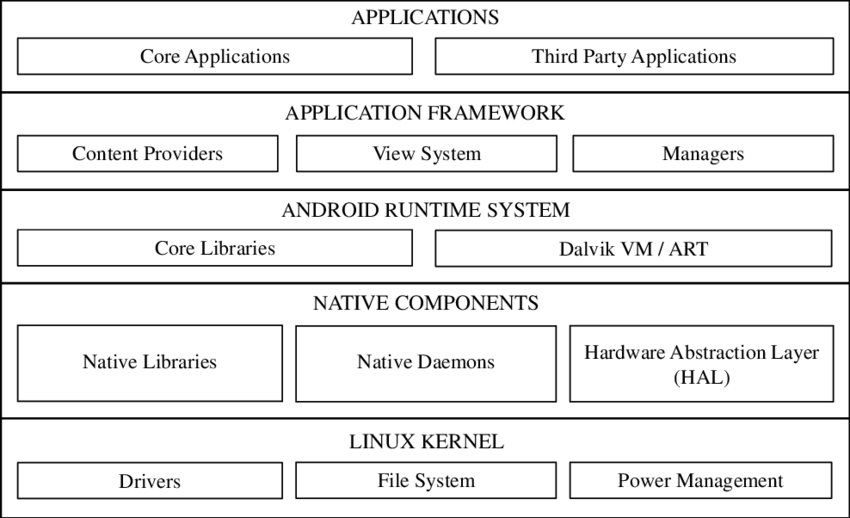
\includegraphics[width=12cm, height=5cm]{Android Operating System Architecture.png}

Linux kernel:
the bottom layer is Linux - Linux 3.6 has approximately 120 patches. This provides an abstraction level between device hardware and includes all the essential hardware drivers such as camera, display etc. In addition, the kernel of the linux is very good at networking and a large array of computer drivers that take the pain out of peripheral hardware interfaces.


\subsection{Android Libraries (Native Components)}

This subsection covers certain Java based libraries that are unique to the development of Android. Examples of libraries in this subsection include application framework libraries, as well as those that enable user interface creation, design illustration, and database access. The following is a description of some main Android libraries available 

Android.app: provides access to the App model and is the main component of all Android apps. 

Android.database: Used to access content providers' published data, and includes SQLite databases

Android.os: provides the main operating system services such as system services ,messages and inter-process communications between applications. 

Android.opengl: The OpenGL ES 3D graphics Java interface to render the API.

Android.widget: components such as buttons, widgets, labels, list views etc.

Android.webkit: A set of classes designed to incorporate Web browsing capabilities into applications.


\subsection{Android Runtime} 
the third section is about the architecture and it's available on the second layer from the bottom. This section provides a key component called Dalvik Virtual Machine which is nearly similar to Java Virtual Machine (JVM) but it's uniquely designed and optimized for Android.

The Dalvik VM uses Linux main features such as multi-threading and memory managementment , which is intrinsic to Java language.
The Dalvik VM allows each Android application to run in it's own process, with Dalvik virtual machine as its own case.

Apart from the main one, the Android runtime also provides a set of core libraries that allow Android application to be written using standard Java programming language.

\subsection{Application Framework}
The Application Framework layer provides applications with many higher-level services in Java class format. Those facilities developing apps.

Action Manager: Manages all facets of the lifecycle and operation stack of an program. 

Content Providers: Allows the publication and sharing of data with other applications. 

Resource Manager: offers access to non-code embedded tools including strings, color preferences, and configurations of the user interface.  

 notification Manager: Allows the user to access updates and feedback from apps. 

System View: An extensible series of views used to construct user interfaces for applications.\cite{8}

\subsection{Applications}

All applications, including the ones that come with Android OS are written at this level. This means a couple important things:
All applications are written in Java, which means they are able to be run on ANY installation of Android OS as .apk. These are hardware independent and are compiled into dex format.
Any software developer can write the same applications as Google. So UI (including the homescreen) can be customized.


\section{\large{Process Management}}

Any android process can be in one of five different states at any time, It's called Process lifespan Hierarchy, from the most important to the least important:

1. Foreground process: The application you are using is considered to be the process in the foreground. Other processes can also be considered primary processes — for instance, if they interact with the process currently in the foreground.\\
2. Visible process: A visible process is not at the foreground but still affects what you have on your mobile screen. For instance, the process in the foreground may be a dialog that allows you to see an application behind it. \\
3. Service process: A service process is not linked to any app on your screen that is visible. In the background, though, it does something like playing music or downloading data in the background.
\\
4. Background process: At present, background processes are not available to the user. They have no effect on the phone use experience. Many background processes are currently under way at any given time. Such processes in the background function as paused apps. They are kept in memory so that you can resume using them quickly when you return to them, but they do not use valuable CPU time.\\ 
5. Empty process: it's  no longer contains info about an app. used to speed up app launches later, it may be kept around as cache files and eventually the system may kill it as needed.

%\subsection{Process Management} 
%Process management in a typical operating system involves many complex data structures and algorithms, but doesn’t go much beyond the level managing the typical process data structure.  Android is similar in that at the base level the control structures look the same.  Similar to this:

%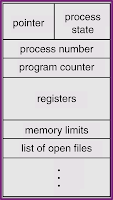
\includegraphics[scale=1]{PCB.png}

%Process Control Block
%This data structure is managed by a standard process management, which is something like this:


%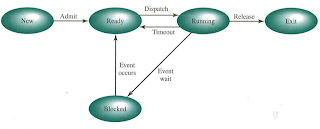
\includegraphics[scale=1]{5StateControl.png}


\subsection{Applications processes}
Android process is the same as process Linux. by necessity, Every .apk installed runs in its own Linux method. by default, There is also 1 thread per process. The main thread has a looper instance for handling messages from the message queue and it calls Looper.loop() in its every iteration of run() method. It's a looper 's job to pop up messages from the message queue and invoke the appropriate methods to handle them. 

Any process gets initiated whenever necessary. Whenever a user or some other system component requests any component (could be a service, activity or intended receiver) that belongs to an apk, if it is not already running, the system spins out a new process for your apk. General processes continue to run until system kills.

\subsection{Process Start up} 
Like many of the Linux-based systems, the bootloader firstly loads the kernel and immediately begins the init process. It generates low-level processes called "daemons". These daemons usually handle low-level hardware interfaces, including the radio interface.

Init cycle begins a process called 'Zygote.'  this is the beginning of the Android platform. The process that initializes the first instance of the Dalvik virtual machine and preloads all the common classed used by the application framework and the various applications. Then it begins listening to future requests to create new vms for handling new device processes. After receiving a new request, it forks itself to build a new process to be a pre-initialized vm instance. 

%\begin{figure}[h]
 %   \centering
  %  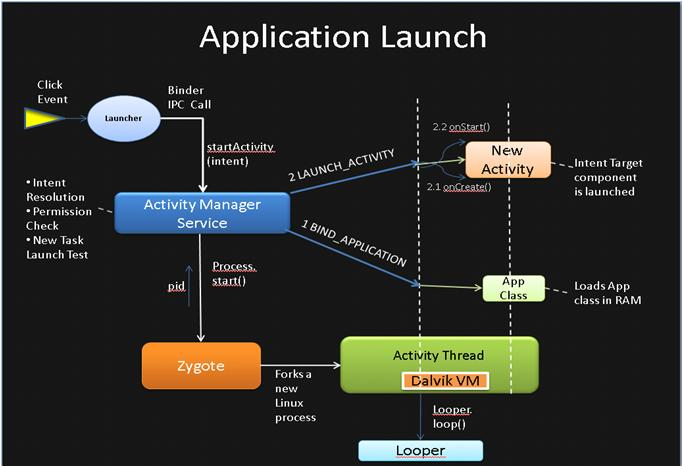
\includegraphics[scale=0.4]{app launch summary.jpg}
    
%\end{figure}
After zygote, the runtime process starts at init.  the zygote initiate  a process called server process. It starts all of the core platform services , e.g. hardware services. At this stage, the system is ready to start the process which displays in the home screen. When a user touches any icon app, the app will be launched and the following things will happen: The click event will be translated into startActivity(intent) call that will be routed to startActivity(intent) call in ActivityManagerService via Binder IPC. ActvityManagerService takes a couple of steps-
\begin{itemize}
\item  the first thing is to gather information about the targeted object by resolveIntent() in PackageManager object.PackageManager.MATCH\_DEFAULT\_ONLY and PackageManager.GET\_SHARED\_LIBRARY\_FILES flags are used as a default choice.
\item The essential information is saved back to the intent object to avoid repeating this step.
\item check if user has enough privileges to invoke the target component of the intent. This is done by calling method GrantUriPermissionLocked(). 
\item If the user has sufficient permissions, ActivityManagerService checks if a new task requires launching of the target activity. The task creation depends on Intent flags such as FLAG\_ACTIVITY\_NEW\_TASK and other flags such as FLAG\_ACTIVITY\_CLEAR\_TOP.
\item  Finally, check if the ProcessRecord is existed  for the process.
\end{itemize}
 
If the ProcessRecord is null, the ActivityManager has to create a new process to instantiate the target component.

There are three distinct phases of process launch :
\begin{enumerate}
\item Process Creation
\item Binding Application
\item Launching Activity 
\end{enumerate}
Process Creation :

The ActivityManagerService will initiate a new process by invoking the startProcessLocked() method that sends arguments to the Zygote process. Zygote forks and calls ZygoteInit.main() which then instantiates the ActivityThread object as well as reterning the pid of the newly created process. 
ActivityThread will start the message loop by calling Looper.prepareLoop() and Looper.loop() afterwards.

The following describes in detail the call sequence  :

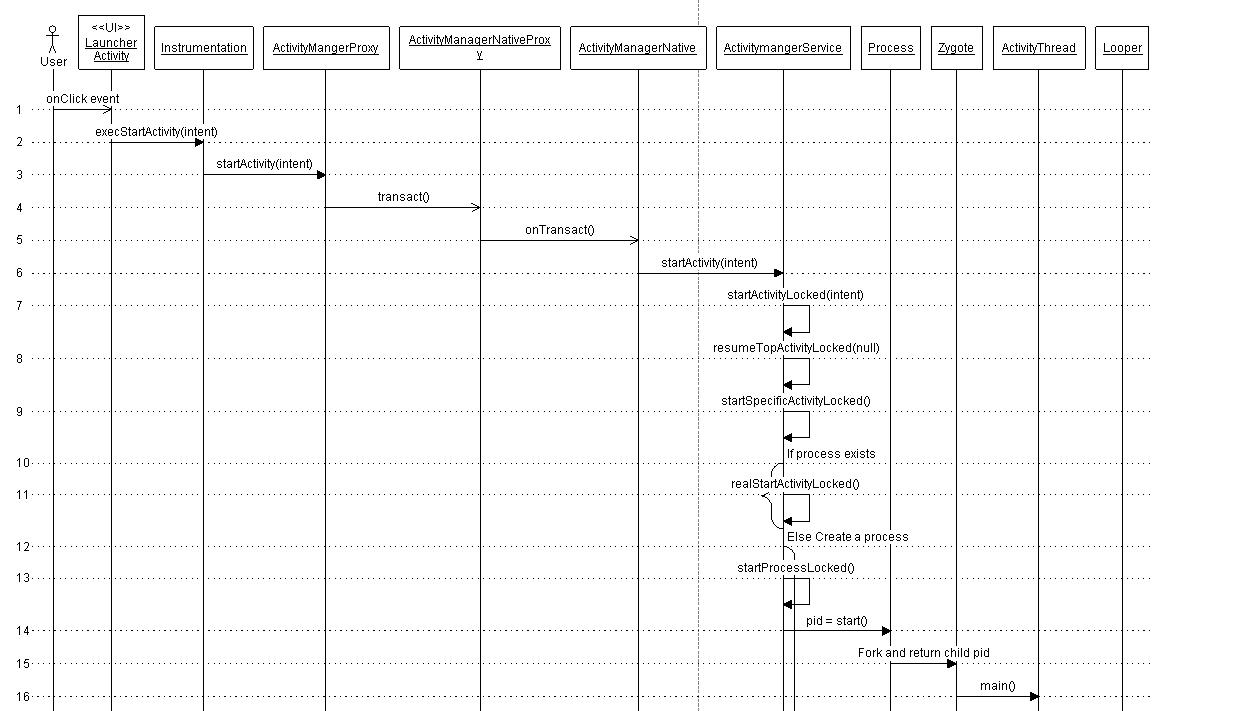
\includegraphics[width=13cm, height=4cm]{App_launch_1.jpg}

Application Binding :

Application Binding: The next step is to add the method to the particular application.This is done by calling bindApplication, the Thread object. This method sends BIND\_APPLICATION message to the queue of messages. This message is collected by the handler object which invokes the handleMessage() method to trigger the specific action of the message  - handleBindApplication(). This method will invoke makeApplication() method which will load separate app specific classes into memory.

This call sequence is shown in following figure.

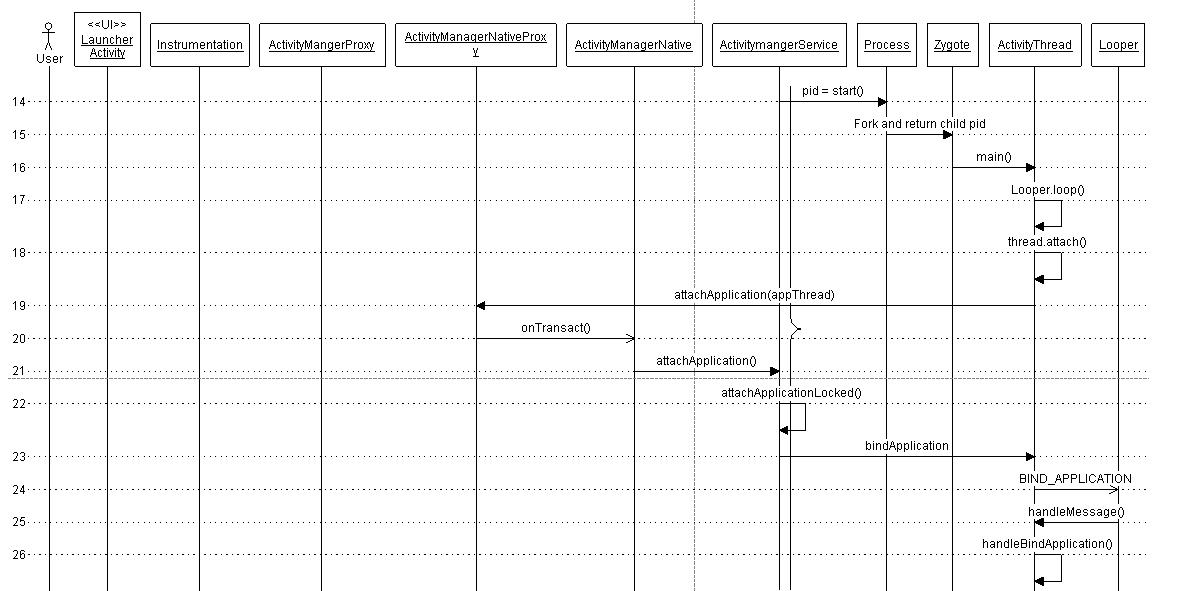
\includegraphics[width=13cm, height=4cm]{App_launch_2.jpg}\\*
 
Activity Launch :

After the previous stage, the system containing the process which is responsible for the application with all application classes are loaded in process's private memory. The call sequence for an operation to start is normal between a newly generated process and an existing one. The actual process of launching starts in realStartActivity() method which calls sheduleLaunchActivity() on the application thread object. This method sends LAUNCH\_ACTIVITY message to the message queue. The message is managed by handleLaunchActivity() method as shown below.
Assuming that user clicks on Video plugin or browser application. the call sequence will launch the activity as shown in the figure.


The Activity starts with onCreate() method call. then comes to foreground with onRestart() call and starts interacting with the user with onStart() call.\\*

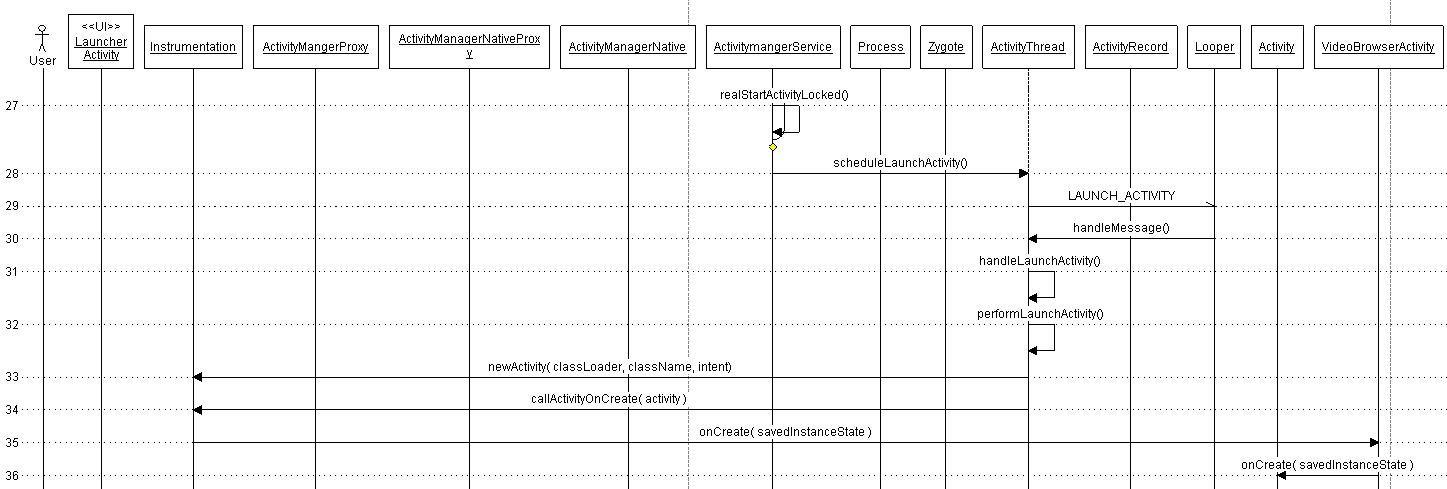
\includegraphics[scale=0.3]{App_launch_3.jpg}

\section{\large{CPU Scheduling Algorithm}} 

Android is Linux based, and uses the scheduling mechanisms of the Linux kernel to determine scheduling policies. This applies to Java code and threads too. 
The Linux schedule strategy combines static and dynamic goals. Processes can be given an initial priority from 19 to -20 (very low to very high priority). This priority will assure that higher priority processes will get more CPU time when when needed. These level are however dynamic, low level priority tasks that do not consume their CPU time will fine their dynamic priority increased. This dynamic behaviour results is an overall better responsiveness.

In terms of dynamic priorities it is ensured that lower priority processes will always have a lower dynamic priority than processes with real-time priorities.

Android uses two main different CPU scheduling mechanisms to schedule process levels 
Linux kernel provides two real-time scheduling algorithms which are SCHED\_FIFO and SCHED\_RR. The main real-time policy is SCHED\_FIFO. Once a SCHED FIFO task begins to run it keeps on running until a higher-priority real-time process willingly yields the cpu, blocks or is preempted. There are no timestamps. 

All other lesser-priority tasks will not be scheduled until the CPU is abandoned. 
Two SCHED FIFO tasks with equivalent priority do not preempt one another, Diffrence between SCHED RR and SCHED FIFO, that these tasks are assigned timestamps depending on their urgency and run until they are completed. Use the SCHED NORMAL scheduling policy for non-real - time tasks. The  Android kernel is designed to allow multi scheduling of real-time operations.

Android uses two different scheduling classes (using linux cgroups)\\ bg\_non\_interactive and default (foreground). The configuration is that \\ bg\_non\_interactive is low priority and can maximum
utilize ~5\% of the cpu (including all background tasks) and foreground ~95\%.
Forground means either an Activity or a service that is started foregound.
\\
Startup Services are always running in bg\_non\_interactive unless they have been raised to foreground scheduling using startForeground (applications are always at foreground level).

 \subsection{JVM thread and process scheduling}
The Android system runs a set of unix processes. Some are native processes, but others are processes that run a Java virtual machine. These processes are normally multi-threaded, and all android threads are native pthreads (no green threads). There are two ways that Calling Thread.setPriority can change priorities. This is part of the standard Java API and contains a value from MIN\_ PRIORITY(1) to MAX\_PRIORITY(10). As all threads are pthreads these priorities will be mapped to unix process priorities (MIN\_PRIORITY being 19 and MAX\_PRIORITY -8).
\begin{center}
 \begin{tabular}{||c c c c||} 
 \hline
 \textbf{Thread.priority} & \textbf{Java name} & \textbf{Android property name      } \textbf{    Unix priority} \\ [0.5ex] 
 \hline\hline
 1 & MIN\_PRIORITY    & ANDROID\_PRIORITY\_LOWEST & 19 \\ 
 \hline
 2 &  & ANDROID\_PRIORITY\_BACKGROUND + 6 &    16 \\
 \hline
 3 &  &  ANDROID\_PRIORITY\_BACKGROUND + 3 & 13 \\
 \hline
 4 &  &  ANDROID\_PRIORITY\_BACKGROUND   &    10 \\
 \hline
 5 & NORM\_PRIORITY   & ANDROID\_PRIORITY\_NORMAL   & 0 \\ 
 \hline
 6 &  & ANDROID\_PRIORITY\_NORMAL - 2 &       -2 \\ 
 \hline
 7 &  &  ANDROID\_PRIORITY\_URGENT\_DISPLAY + 3   & -5 \\
 \hline
 8 &  &  ANDROID\_PRIORITY\_URGENT\_DISPLAY + 2  &  -6 \\
 \hline
 9 & MAX\_PRIORITY    & ANDROID\_PRIORITY\_URGENT\_DISPLAY&        -8 \\ 
 \hline
 
\end{tabular}
\end{center}

The second way to set priorities is to call android.os.Process.setThreadPriority(). This allows to set the pririty to higer priorities for that
Declare: in your AndroidManifest and call Process.setThreadPriority()

frameworks/base/include/utils/threads.h\\
    ANDROID\_PRIORITY\_LOWEST         =  20,\\

    /* use for background tasks */\\
    ANDROID\_PRIORITY\_BACKGROUND     =  12,\\

    /* most threads run at normal priority */\\
    ANDROID\_PRIORITY\_NORMAL         =   0,\\

    /* threads currently running a UI that the user is interacting with */\\
    ANDROID\_PRIORITY\_FOREGROUND     =  -2,\\

    /* the main UI thread has a slightly more favorable priority *\\
    ANDROID\_PRIORITY\_DISPLAY        =  -4,\\
    /* ui service treads might want to run at a urgent display (uncommon) */\\
    ANDROID\_PRIORITY\_URGENT\_DISPLAY =  -8,\\

    /* all normal audio threads */\\
    ANDROID\_PRIORITY\_AUDIO          = -14,

    /* service audio threads (uncommon) */\\
    ANDROID\_PRIORITY\_URGENT\_AUDIO   = -19,\\

    /* regular process  not allowed to use this level */\\
    ANDROID\_PRIORITY\_HIGHEST        = -20,

\section{\large{Memory Management}}
The Android architecture runs on the idea that any free memory is wasted(unused) memory. It's just struggling to fill all of the available memory. The system keeps all apps in the memory after they've been closed so the user can switch back to the closed apps at any time. Android devices often run with very little free memory, for this reason. Memory management is essential for proper allocation of memory between important system processes and multiple user applications.   

The fundamentals of how Android allocates memory for the device and user applications are covered in the following section. It also describes how the operating system responds to circumstances with low memory situations.

\subsection{Memory pages}  
RAM is fractured into pages. Every page is usually 4 KB of memory. 
Pages are either considered safe, or licensed. Unused RAM is considered as a Free Pages. The pages used are RAMs that the program regularly uses, which are divided into the following categories:
\begin{itemize}
	\item Cached: Memory backed by a file on storage (for example, code or memory-mapped files). There are two types of cached memory
	
	\begin{itemize}
    	\item Private: Owned by one process and not shared    
    	
    	\begin{itemize}
    	\item Clean: Unmodified copy of a file may be removed to maximize free memory

        \item Dirty: Modified copy of the file to storage; can be moved to or compressed to zRAM to increase free memory

    \end{itemize}
        
    \end{itemize}
	
    
    \begin{itemize}
    \item Shared: Used by multiple processes

     \begin{itemize}
    	\item Clean: Unmodified copy of the file can be removed to increase free memory.

        \item Dirty:Changed storage copy of the file; allows changes to be written back to the storage file to boost free memory.
        \end{itemize}
    \end{itemize}
    
    \item Anonymous: Memory not backed by a file on storage
     \begin{itemize}
    	\item Dirty: Can be moved/compressed in zRAM to increase free memory
       
    \end{itemize}
\end{itemize}

Clean Pages contain an same copy of a stored file (or part of a file). A clean page becomes a dirty page because it no longer contains an exact copy of the file like,the product of an application process . Clean pages can be removed because the data from the database can still be regenerated; dirty pages can not be removed, or data will be lost. 
Within time, the proportions of free and used pages differ as the program actively manages RAM. The concepts presented in this section are key for the management of low-memory situations. Those are described in greater depth in the next section \cite{9}

\subsection{low memory management}

Android has two main techniques to counter low memory situations: the kernel swap daemon and low-memory killer.

 \subsubsection{kernel swap daemon} 
The kernel swap daemon also known as (kswapd) is a main part of the kernel and transform the memory used to free memory. The kswapd will become active when the free memory of the phone is running low. Once free memory slips below the small threshold, kswapd begins to restore memory. When free memory reaches a high threshold, kswapd stops retrieving memory.

\begin{figure}[h]
    \centering
    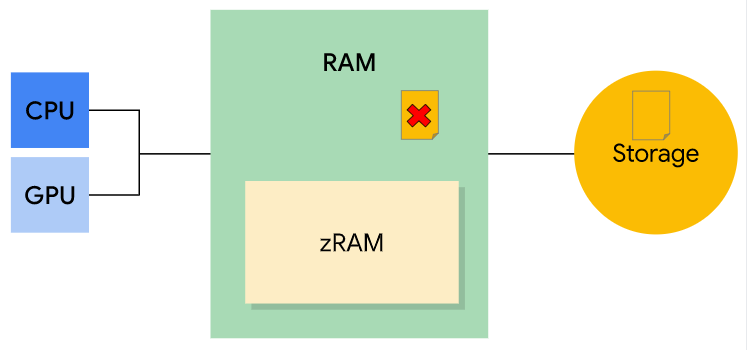
\includegraphics[scale=0.4]{ram1.png}
    \caption{Clean page, backed by storage, deleted}
    \label{fig:mesh1}
\end{figure} 

kernel swap daemon can retrieve clean pages because they are backed up in storage without modification. If a process attempts to retrieve a deleted clean page, the kernal will copy the page from main storage to the RAM. This method is referred to as demand paging.

\begin{figure}[h]
    \centering
    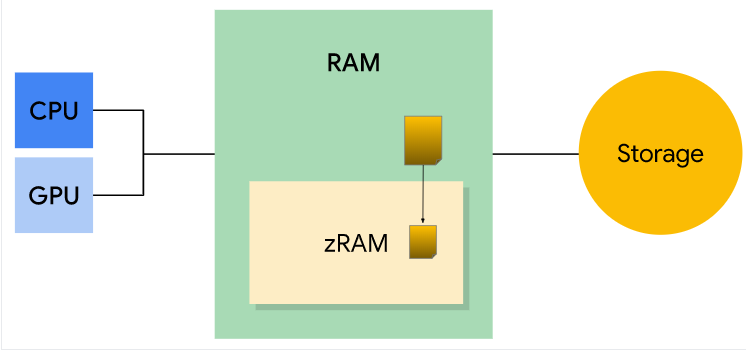
\includegraphics[scale=0.4]{ram2.png}
    \caption{Dirty page moved to zRAM and compressed}
   
\end{figure}
kernel swap daemon can redirect cached and anonymous private dirty pages into zRAM,(place of compression). This frees up the available memory in the RAM. When the process attempts to move a dirty page in the zRAM, the page will be uncompressed and will return to RAM. If the process related with a compressed page is killed, the page also will be deleted from zRAM. 

the system may start killing processes. If the amount of free memory went down to a serious level.
    
 \subsubsection{Low-memory killer} 

if Kswapd has not been able to free enough memory for the system. In this case, the system uses TrimMemory() to tell the app that the memory is at low level and that it should minimize it's memory allocation. If it's not enough, the kernel will use low-memory killer (LMK) to start killing processes(considering priority) to free the memory.
LMK uses a score called "out of memory" to prioritize running processes to decide the processes that will be kill. Background processes are killed first, and system processes killed last.

\subsection{Garbage collection} 
The managed memory environment, such as the Dalvik virtual machine or ART (after Android 5.0), it keeps track of all memory allocations. When it says that the program is no longer in the memory, it will be released to the heap, without any interference from the programmer. The method for restoring unused memory in a controlled memory is well known as garbage collection. Garbage collecting has two objectives: to identify the objects in the memory that can not be retrieved in the future and to recover the resources used by such objects. \\

The heap of the Android's memory is a generational one, meaning that there are various seals of allocations that it records, depending on the projected existence and scale of the object being allocated. Newly allocated objects, for example, belong to the Young Generation. If the object stays alive long enough, it may be transferred to an older generation, and then transferred to a permanent generation.\\ 

That generation of heaps has its limit. Whenever a generation starts filling up, the machine will execute the garbage collection to free the memory. The period of the garbage collection depends on the group of objects it gathers and how many active objects there are in each generation.\\

The system has a set of criteria in place to determine when to excute garbage collector. When the conditions are met, the system will stop executing the process and starts garbage collection. If garbage collection happens in the midst of an intense processing cycle, such as an playing games or during music playback, the processing time can be increased.\\


\subsubsection{Share memory} 
Android is always trying to share available RAM across all available processes in order for everything to fit in ram. This can be done in the next ways:\\ 

Each new application process is forked by an existing process called Zygote. The Zygote cycle begins when the machine starts up and loads the main frameworks and tools.  To start any new process, the system begins to forks Zygote process, it runs the app code in the new process. This technique permits most of the RAM pages to be assigned to the framework code
also it allows the available resources to be shared all across  app processes. \\

Most of the static data is mmapped in a process. This method allows all required data to be exchanged between systems, and allows it to be paged out as appropriate.
\section{\large{Virtual memory}}
Android Runtime (ART) -introduced to android 4.4 as a beta feature and became final in android 5.0 - and Dalvik virtual machines use paging and memory mapping to manage memory. 
The main visible benefit of this strategy is that programs can be greater than physical memory and run normally. Virtual memory is usually for two main purposes. First, it allows the physical memory to be extended by the disk. Second , it protects memory, because every virtual memory address will be translated to a physical address. 
The following situations arise when the whole program is not needed to be fully loaded into the main memory.\cite{7}
\begin{itemize}
\item User written error handling routines are only used when a data or computation error has occurred.
\item Such software functions may not used frequently.
\item A fixed amount of address space is assigned to many tables even an only small amount of the table is used. So, the ability to execute a program that uses partial amount of memory would counterbalanced many of the benefits. 
\item lesser amount of I / Os is needed to load or swap the memory of each user program.
\end{itemize}

\subsection{Page Replacement Algorithm}

Page Replacement Algorithms are the methods used by the Operating System to determine which memory pages to move or write to the disk when any memory page has to be allocated. Paging occurs whenever a page error happens and a free memory page can not be used for the purpose of allocation accounting. it occurs due to that pages are not available or that the number of free pages is less than the required pages. 

If the page that has been chosen for replacement and has been paged out is referenced again, it needs to be read from the disk, and that involves I / O completion. This method determines the efficiency of any page replacement algorithm: the longer time you wait for the page-ins, the faster the algorithm.

A page replacement algorithm looks at the minimal details on accessing the pages given by the hardware and tries to choose which pages to be replaced to reduce the overall amount of pages lost while matching them with the costs of primary storage and processing time of the algorithm itself. 
There are a number of common page replacement algorithms. Some of them are explained in the following subsections.

\subsection{First In First Out (FIFO) algorithm}

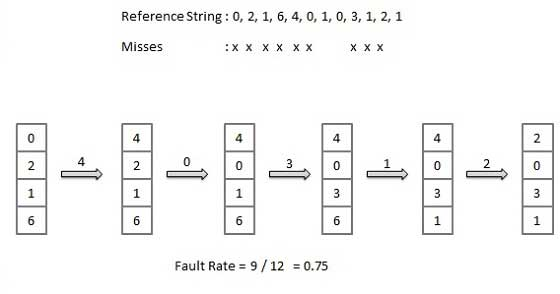
\includegraphics[width=10cm, height=4cm]{fifo.jpg}\\
The oldest page in the main memory is the one that will be picked for replacment. It's Easy to implement, new pages are added to the head and page replacments occurs from the tail

\subsection{Optimal Page algorithm}
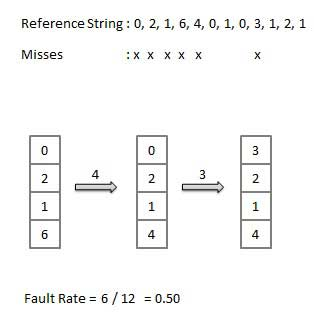
\includegraphics[width=10cm, height=4cm]{opr.jpg}\\
This algorithm has the lowest page-fault rate of all algorithms. it's also called OPT or MIN. It depend on Replacing the page that will not be used for the longest amount of time. Use the time when a page is not used.
\subsection{Least Recently Used}
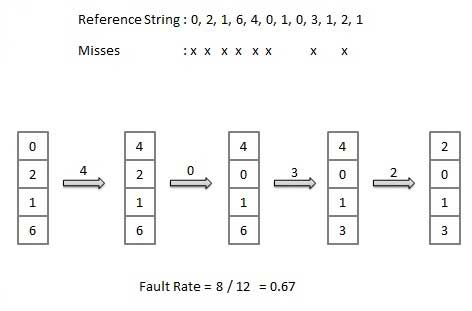
\includegraphics[width=10cm, height=4cm]{lru.jpg}\\

Any Page which hasn't been used for the longest period of time in main memory will be selected for replacement.
\section{Conclusion}
Android is a much more flexible operating system than iOS  it's truly open, free development platform based on linux and open source. Android has grown rapidly over the years to become the most widely used smartphone operating system in the world. It's because Android doesn't release 1 phone from 1 company with 1 new OS a year, but countless phones from a variety of companies, all year round, are slowly evolving day-by-day. Android's ability to customize is unparalleled relative to Apple's apps, enabling users to modify and configure nearly any part of Android that other iPhone users will never conceive about. Android is exceptional and incomparable to many smartphone operating systems.

%% The Appendices part is started with the command \appendix;
%% appendix sections are then done as normal sections
%% \appendix

%% \section{}
%% \label{}

%% References
%%
%% Following citation commands can be used in the body text:
%% Usage of \cite is as follows:
%%   \cite{key}          ==>>  [#]
%%   \cite[chap. 2]{key} ==>>  [#, chap. 2]
%%   \citet{key}         ==>>  Author [#]

%% References with bibTeX database:
\begin{thebibliography}{10}
\bibitem{1} 
Alabaster, J. (2020). Android founder: We aimed to make a camera OS. Retrieved 6 June 2020, from https://www.pcworld.com/article/2034723/android-founder-we-aimed-to-make-a-camera-os.html
\textit{(Alabaster, 2020)}. 
\bibitem{2} 
(2020). Retrieved 6 June 2020, from http://www.openhandsetalliance.com/oha\_faq.html
%\textit{Zur Elektrodynamik bewegter K{\"o}rper}. (German) 
%[\textit{On the electrodynamics of moving bodies}]. 
%Annalen der Physik, 322(10):891–921, 1905.
\bibitem{3} 
Menon, M. (2020). Android Nougat: Here’s why Google names the OS after sweets. Retrieved 7 June 2020, from https://indianexpress.com/article/lifestyle/food-wine/from-donut-to-nougat-why-are-android-versions-named-after-sweets-2887237/

\bibitem {4}
Stallings, W. (2014). Operating Systems: Internals and Design Principles, Global Edition (9th ed.). Pearson.
\bibitem {5}
Tanenbaum, A., \& Boschung, H. (2014). Modern operating systems (4th ed.). Pearson.
\bibitem {6}
Arpaci-Dusseau, R. (2015). Operating Systems: Three Easy Pieces (1st ed., p. 211). Arpaci-Dusseau Books.
\bibitem {7}
McHoes, A., \& M.Flynn, I. (2017). Understanding operating systems (8th ed., Ch.16).
\bibitem {8}
Burnette, E. (2015). Hello, Android (4th ed.). Pragmatic programmers.
\bibitem {9}

Deitel, H., \& Deitel, P. (2014). Android (3rd ed.). Harlow, United Kingdom: Pearson Education Canada.


\end{thebibliography}

\bibliographystyle{apacite}

\bibliography{references.bib}





%% Authors are advised to submit their bibtex database files. They are
%% requested to list a bibtex style file in the manuscript if they do
%% not want to use model1-num-names.bst.
%% References without bibTeX database:

% \begin{thebibliography}{00}

%% \bibitem must have the following form:
%%   \bibitem{key}...
%%

% \bibitem{}

% \end{thebibliography}

 






\end{document}

%%
%% End of file `elsarticle-template-1-num.tex'.
